\documentclass[11pt]{article}

% ---------- packages ----------
\usepackage[utf8]{inputenc}
\usepackage[T1]{fontenc}
\usepackage{lmodern}
\usepackage[a4paper,margin=1in]{geometry}
\usepackage{amsmath,amssymb}
\usepackage{bm}
\usepackage{booktabs}
\usepackage{tabularx}
\usepackage{array}
\usepackage{microtype}
\usepackage{enumitem}
\usepackage{xcolor}
\usepackage{titlesec}
\usepackage{graphicx}
\usepackage{tikz}
\usetikzlibrary{positioning,arrows.meta,calc,patterns,fit,backgrounds,shapes.geometric,decorations.pathreplacing}
\usepackage{float}
\usepackage{caption}
\usepackage{listings}
\usepackage[hidelinks,colorlinks=true,linkcolor=teal!60!black,citecolor=teal!60!black,urlcolor=teal!60!black]{hyperref}

% ---------- styling ----------
\definecolor{accent}{RGB}{20,90,90}     % teal -- state / fine net
\definecolor{accent2}{RGB}{180,95,30}   % orange -- operators / halo
\definecolor{accent3}{RGB}{70,70,140}   % indigo -- coarse path
\definecolor{boxbg}{RGB}{245,247,247}
\definecolor{solidc}{RGB}{120,120,120}
\titleformat{\section}{\large\bfseries\color{accent}}{\thesection}{0.6em}{}
\titleformat{\subsection}{\normalsize\bfseries}{\thesubsection}{0.6em}{}
\setlist{itemsep=2pt,topsep=3pt,parsep=0pt}
\renewcommand{\arraystretch}{1.25}
\newcolumntype{Y}{>{\raggedright\arraybackslash}X}

% ---------- algorithm float + listings pseudocode ----------
\newfloat{algorithm}{tbp}{loa}
\floatname{algorithm}{Algorithm}
\lstdefinestyle{pseudo}{
  basicstyle=\ttfamily\small,
  keywordstyle=\color{accent}\bfseries,
  keywordstyle=[2]\color{accent2}\bfseries,
  commentstyle=\itshape\color{gray},
  morekeywords={for,each,if,else,then,return,while,do,end,Input,Output,Require,Ensure,with},
  morekeywords=[2]{CoarseStep,Restrict,Prolong,Blend,Predict,Project,Tile,Merge,Pad,Crop},
  columns=fullflexible,
  keepspaces=true,
  showstringspaces=false,
  frame=none,
  xleftmargin=1.2em,
  aboveskip=2pt,belowskip=2pt,
}

% ---------- math shortcuts ----------
\newcommand{\R}{\mathbb{R}}
\newcommand{\Rop}{\mathcal{R}}
\newcommand{\Eop}{\mathcal{E}}
\newcommand{\Gfine}{\mathcal{G}_{\Phi}}
\newcommand{\Gcoarse}{\bar{\mathcal{G}}_{\Psi}}
\newcommand{\F}{\mathcal{F}}
\newcommand{\code}[1]{\texttt{#1}}

% ---------- reusable tikz styles ----------
\tikzset{
  blk/.style={draw,rounded corners,align=center,font=\small,fill=boxbg,minimum height=8mm,inner sep=3pt},
  net/.style={blk,fill=accent!15,draw=accent},
  cnet/.style={blk,fill=accent3!15,draw=accent3},
  op/.style={blk,fill=accent2!12,draw=accent2},
  io/.style={align=center,font=\small\bfseries},
  ar/.style={-{Stealth[length=2.4mm]},thick},
  car/.style={-{Stealth[length=2.4mm]},thick,accent3},
}

\title{\vspace{-1.2cm}\textbf{A Domain-Decomposed Neural Surrogate for Urban Flow}\\[3pt]
\large Design, implementation, and usage in \texttt{pyurbanair}}
\author{Research note --- \texttt{pyurbanair} / neural surrogates}
\date{\today}

\begin{document}
\maketitle
\vspace{-0.4cm}

\begin{abstract}
\noindent
We describe a two-level, overlapping \emph{domain-decomposed} neural surrogate for
one-step prediction of urban large-eddy-simulation (LES) flow fields, and its
concrete implementation in the \texttt{pyurbanair} code base. A single shared
convolutional network is tiled over overlapping subdomains and blended back with a
smooth partition of unity, while a cheap coarse network supplies each tile with a
global, low-resolution \emph{context} field that restores the long-range coupling
a purely local model would lose. The decisive design choice is that the entire
decomposition is \emph{embedded inside one \texttt{nn.Module}}: the model keeps the
ordinary full-grid contract \code{forward(state, params, geometry)\,$\to$\,state\_next},
so it trains with the existing trainer and runs through the existing forward-model
and data-assimilation machinery with no changes to either. Because the trained
quantity is a fixed-size \emph{patch} rather than a fixed global grid, one trained
model runs on any grid with the same cell spacing. We give the full mathematical
setup, the partition-of-unity construction (including a genuine periodic
wrap-around for the spanwise direction), the two training routes --- a plain
mean-squared drop-in and a four-term patch objective with interface, divergence and
coarse-supervision penalties --- and the software layout (modules, Hydra
configuration groups, and tests). The document is figure-heavy by design: each step
of the pipeline is illustrated.
\end{abstract}

% =====================================================================
\section{Introduction}\label{sec:intro}

\texttt{pyurbanair} learns cheap surrogates of computational-fluid-dynamics (CFD)
forward models for urban wind and dispersion. The existing surrogate is a single
translation-equivariant 3D convolutional network $\Gfine$ that maps a state
$\bm S_t$, an inflow parameter vector $\bm p_t$ and a static geometry mask $\bm m$
to the next state, $\Gfine(\bm S_t,\bm p_t,\bm m)\approx\bm S_{t+1}$, applied to the
\emph{whole} grid at once. Two pressures motivate going beyond whole-grid
application:

\begin{enumerate}
\item \textbf{Memory and resolution.} A whole-grid 3D network's activation memory
grows with the domain. Training at city scale, or at finer resolution, eventually
does not fit. Tiling a fixed-size patch decouples the trainable footprint from the
domain size.
\item \textbf{Reuse across domains.} A whole-grid network is welded to the exact
grid it trained on. We would prefer a model whose invariant is a physical patch, so
the same weights apply to a larger or differently-shaped domain at the same
resolution.
\end{enumerate}

Domain decomposition is the classical remedy: cover the domain with overlapping
subdomains, solve locally, and reconcile the overlaps. The one subtlety for
incompressible flow is that pressure couples the whole field instantaneously (the
pressure Poisson equation $\nabla^2 p=-\nabla\!\cdot(\bm u\!\cdot\!\nabla\bm u)$ is
elliptic), so a purely local tiling cannot represent global effects within a single
step. Following standard multilevel domain-decomposition practice
\cite{dryja1994smalloverlap,dolean2024multilevel,li2020mgno}, we add a cheap coarse
level that carries exactly this global coupling.

\paragraph{Contributions and design principle.}
This note documents the implementation, not a new algorithm. Its one firm principle
is \emph{transparency to the rest of the stack}: the decomposition is hidden inside
the model, so every caller --- trainer, autoregressive rollout, ensemble, and the
ensemble-smoother data assimilation --- sees the same interface as any other
architecture (Section~\ref{sec:contract}). On top of that we contribute: a uniform,
padding-based tiling with a normalized partition of unity that is exact across a
\emph{periodic} seam (Section~\ref{sec:geometry}); a minimal, back-compatible
widening of the existing UNet so it can ingest the coarse context
(Section~\ref{sec:fine}); a forward model whose domain check is relaxed to a
cell-spacing invariant so the global grid becomes a free parameter
(Section~\ref{sec:flexible}); and two interchangeable training routes wired as
configuration groups (Section~\ref{sec:training}).

Figure~\ref{fig:overview} is the whole method on one page; the rest of the document
expands each block.

% ---- HERO FIGURE ----
\begin{figure}[t]
\centering
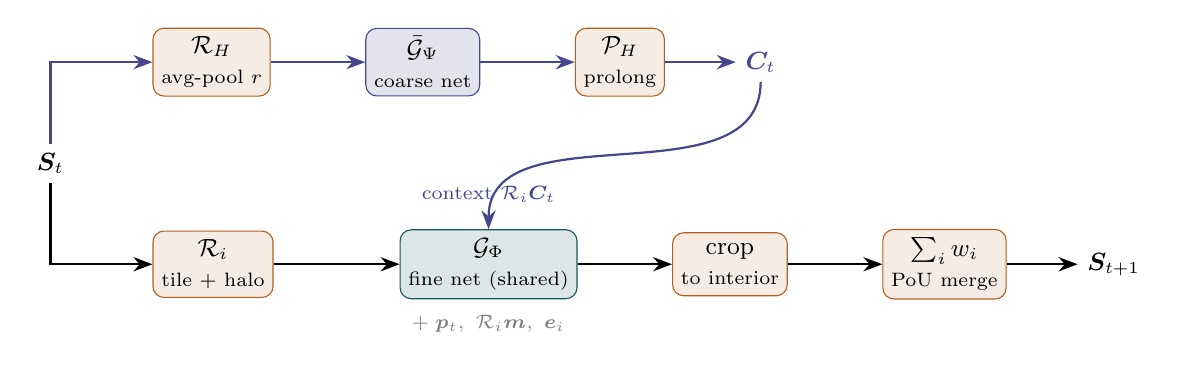
\begin{tikzpicture}[node distance=7mm and 12mm]
  \node[io] (S) {$\bm S_t$};
  % coarse path (top, indigo)
  \node[op,above right=6mm and 10mm of S] (DH) {$\Rop_H$\\\scriptsize avg-pool $r$};
  \node[cnet,right=of DH] (GC) {$\Gcoarse$\\\scriptsize coarse net};
  \node[op,right=of GC] (PH) {$\mathcal P_H$\\\scriptsize prolong};
  \node[io,right=9mm of PH,accent3] (C) {$\bm C_t$};
  % fine path (bottom, teal)
  \node[op,below right=6mm and 10mm of S] (Ri) {$\Rop_i$\\\scriptsize tile $+$ halo};
  \node[net,right=16mm of Ri] (GF) {$\Gfine$\\\scriptsize fine net (shared)};
  \node[op,right=of GF] (cr) {crop\\\scriptsize to interior};
  \node[op,right=of cr] (BL) {$\sum_i w_i$\\\scriptsize PoU merge};
  \node[io,right=9mm of BL] (Snext) {$\bm S_{t+1}$};
  % arrows coarse
  \draw[car] (S) |- (DH);
  \draw[car] (DH) -- (GC);
  \draw[car] (GC) -- (PH);
  \draw[car] (PH) -- (C);
  % arrows fine
  \draw[ar] (S) |- (Ri);
  \draw[ar] (Ri) -- (GF);
  \draw[ar] (GF) -- (cr);
  \draw[ar] (cr) -- (BL);
  \draw[ar] (BL) -- (Snext);
  % context injection
  \draw[car] (C) to[out=-90,in=90] (GF.north);
  \node[font=\scriptsize,accent3,anchor=south] at ($(GF.north)+(0,0.22)$) {context $\Rop_i\bm C_t$};
  \node[font=\scriptsize,gray,anchor=north] at ($(GF.south)+(0,-0.08)$) {$+\;\bm p_t,\ \Rop_i\bm m,\ \bm e_i$};
\end{tikzpicture}
\caption{\textbf{One step of the two-level domain-decomposed update.}
\emph{Top (indigo):} a cheap coarse predictor average-pools the state by a factor
$r$, takes one low-resolution step, and prolongs the result to a fine-grid
\emph{context} field $\bm C_t$ that carries global coupling. \emph{Bottom (teal):}
the field is tiled into overlapping blocks; a single shared fine network predicts a
residual per patch from the patch state, its halo, geometry, parameters, the
restricted context $\Rop_i\bm C_t$ and a positional encoding $\bm e_i$; the outputs
are cropped to their interiors and blended by a partition of unity into the next
state $\bm S_{t+1}$. The whole diagram is one call of \code{DomainDecomposed.forward}.}
\label{fig:overview}
\end{figure}

% =====================================================================
\section{Problem setup and notation}\label{sec:notation}

The discretized state on the full grid is
$\bm S_t\in\R^{C\times N_z\times N_y\times N_x}$, with $C$ channels (the velocity
components $u,v,w$, and optionally pressure $p$), a static binary geometry mask
$\bm m\in\{0,1\}^{N_z\times N_y\times N_x}$ ($1=$ fluid, $0=$ solid), and an inflow
parameter vector $\bm p_t\in\R^{P}$. The reference LES solver advances the state by
one output step,
\begin{equation}
\bm S_{t+1}=\F(\bm S_t,\bm p_t,\bm m),
\label{eq:truth}
\end{equation}
and the surrogate learns a cheap approximation of $\F$. Tensors follow the PyTorch
layout $(B,C,z,y,x)$ with batch dimension $B$; the geometry enters as one extra
channel and the network output is multiplied by the mask so solid cells stay
exactly zero.

\paragraph{Subdomains, interiors, halos.}
Cover the grid by $M$ overlapping subdomains. Each has an \emph{interior} block
$\Omega_i^\circ$ of shape $n\times n\times n$ that the network is responsible for
predicting, and an \emph{extended} block $\hat\Omega_i$ of shape $(n+2h)^3$ obtained
by growing the interior by a \emph{halo} of width $h$ on every side. The halo cells
are read as input context but their predictions --- which lack their own neighbours
--- are discarded. Define the two linear operators
\begin{equation}
\Rop_i:\R^{C\times N_z\times N_y\times N_x}\to\R^{C\times(n+2h)^3},
\qquad
\Eop_i:\R^{C\times n^3}\to\R^{C\times N_z\times N_y\times N_x},
\label{eq:restrict-extend}
\end{equation}
where $\Rop_i$ \emph{restricts} the global field to the extended block (this is
where a subdomain reads its halo from its neighbours), and $\Eop_i$ \emph{extends}
an interior-block field back onto the global grid, zero outside $\Omega_i^\circ$.
Figure~\ref{fig:decomp} shows the geometry. Interior blocks tile the domain; the
extended blocks overlap.

\begin{figure}[t]
\centering
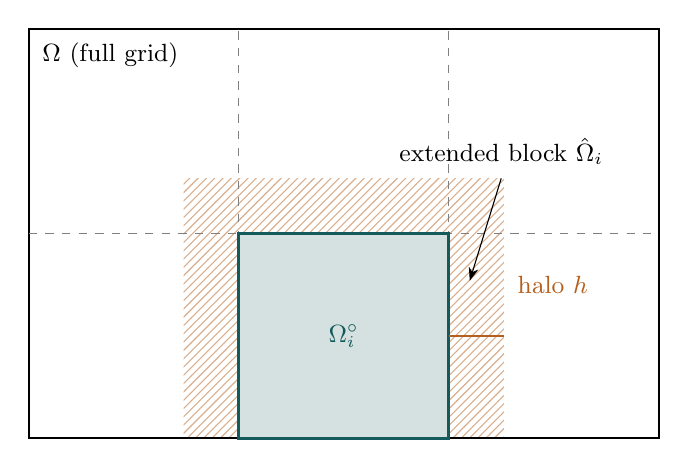
\begin{tikzpicture}[scale=1.0]
  \draw[thick] (0,0) rectangle (8,5.2);
  \node[anchor=north west] at (0.05,5.15) {\small $\Omega$ (full grid)};
  \foreach \x in {2.6667,5.3333} {\draw[gray,dashed] (\x,0) -- (\x,5.2);}
  \foreach \y in {2.6} {\draw[gray,dashed] (0,\y) -- (8,\y);}
  \begin{scope}[on background layer]
    \fill[pattern=north east lines, pattern color=accent2!50]
      (2.6667-0.7,0) rectangle (5.3333+0.7,2.6+0.7);
  \end{scope}
  \fill[accent!18] (2.6667,0) rectangle (5.3333,2.6);
  \draw[accent,very thick] (2.6667,0) rectangle (5.3333,2.6);
  \node[accent,font=\small\bfseries] at (4,1.3) {$\Omega_i^\circ$};
  \draw[accent2,thick] (5.3333,1.3) -- (5.3333+0.7,1.3);
  \node[accent2,font=\small,anchor=west] at (5.3333+0.75,1.95) {halo $h$};
  \node[font=\small,anchor=south] at (6.0,2.6+0.75) {extended block $\hat\Omega_i$};
  \draw[->,>=Stealth] (6.0,2.6+0.7) -- (5.6,2.0);
\end{tikzpicture}
\caption{\textbf{Overlapping decomposition.} Each subdomain predicts its interior
block $\Omega_i^\circ$ (teal) but reads inputs from the larger extended block
$\hat\Omega_i$ (hatched), which adds a halo of width $h$ taken from neighbouring
cells. Interior blocks tile the domain edge-to-edge; extended blocks overlap by
$2h$.}
\label{fig:decomp}
\end{figure}

% =====================================================================
\section{Domain-decomposition geometry}\label{sec:geometry}

This section fixes how the grid is tiled, how the partition-of-unity weights are
built, and how periodicity is handled. All of this lives in one I/O-free helper,
\code{DomainDecomposition} (file \code{decomposition.py}), which caches a tiling
\emph{plan} per global grid shape so a single model instance can serve different
grids.

\subsection{Uniform tiling by padding}\label{sec:tiling}

Rather than clip extended blocks at the global boundary (which would make them
ragged and break a single batched network call), we \emph{pad} the field so every
block is the same shape. Each non-periodic axis is first padded up to a multiple of
$n$, so the interiors tile it exactly; then a halo of width $h$ is padded on every
side. Boundary halos use replicate padding by default (a sane Neumann-like
extension; zero is also available), and \emph{circular} padding on periodic axes
(Section~\ref{sec:periodic}). Every extended block is then exactly $(n+2h)^3$, the
$M$ blocks stack into one tensor of shape $(B\,M,C,n+2h,n+2h,n+2h)$, and a single
forward pass evaluates them all. After merging, the result is cropped back to the
exact original $(N_z,N_y,N_x)$. Figure~\ref{fig:tiling} shows the two padding bands
along one axis.

\begin{figure}[t]
\centering
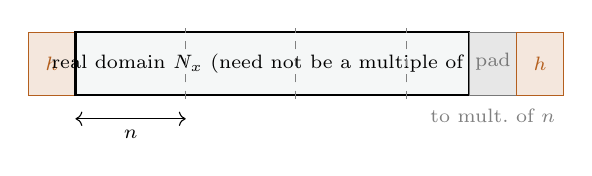
\begin{tikzpicture}[ar/.style={-{Stealth[length=2mm]},thick}]
  \def\n{1.4}
  \draw[fill=accent2!15,draw=accent2] (-0.6,0) rectangle (0,0.8);
  \node[font=\scriptsize,accent2] at (-0.3,0.4) {$h$};
  \draw[thick,fill=boxbg] (0,0) rectangle (5.0,0.8);
  \node[font=\scriptsize] at (2.5,0.4) {real domain $N_x$ (need not be a multiple of $n$)};
  \draw[fill=solidc!18,draw=solidc] (5.0,0) rectangle (5.6,0.8);
  \node[font=\scriptsize,solidc] at (5.3,0.42) {pad};
  \draw[fill=accent2!15,draw=accent2] (5.6,0) rectangle (6.2,0.8);
  \node[font=\scriptsize,accent2] at (5.9,0.4) {$h$};
  \foreach \i in {1,2,3} {\draw[gray,dashed] (\i*\n,-0.05) -- (\i*\n,0.85);}
  \draw[<->] (0,-0.3) -- (\n,-0.3);
  \node[font=\scriptsize,anchor=north] at (0.5*\n,-0.32) {$n$};
  \node[font=\scriptsize,anchor=north,gray] at (5.3,-0.05) {to mult.\ of $n$};
\end{tikzpicture}
\caption{\textbf{Uniform tiling by padding (one axis).} A non-periodic axis is
padded up to a multiple of the interior size $n$ (grey, replicate/zero) so interior
tiles (dashed, width $n$) cover it exactly, then a halo of width $h$ (orange) is
added on each side. Every extended block is then a uniform $(n+2h)$ along this axis,
which lets all $M$ patches batch into one network call. The final merged field is
cropped back to $N_x$.}
\label{fig:tiling}
\end{figure}

\subsection{Partition of unity}\label{sec:pou}

The interior predictions are recombined with smooth window functions
$w_i:\Omega\to[0,1]$ that form a \emph{partition of unity}:
\begin{equation}
\sum_{i=1}^{M} w_i(\bm x)=1\quad\text{for every grid point }\bm x.
\label{eq:pou}
\end{equation}
Each window is a separable Hann taper that ramps from $0$ at the block edge to $1$ a
distance $\delta$ (the \emph{taper} width, $\delta\le h$) inside. Crucially, the
windows are defined on blocks of size $n+2\delta$ --- the interior grown by the
taper band on each side --- so neighbouring windows genuinely overlap by $2\delta$
and their ramps add. (Windows on the strict interior $n$ would be disjoint and
\eqref{eq:pou} would hold only trivially, with no blending.) After construction the
windows are divided by their overlap sum $S(\bm x)=\sum_j w_j(\bm x)$ once, which
makes \eqref{eq:pou} exact everywhere, including at the domain boundary where a tile
has fewer neighbours. Figure~\ref{fig:pou} shows the 1D picture.

\begin{figure}[t]
\centering
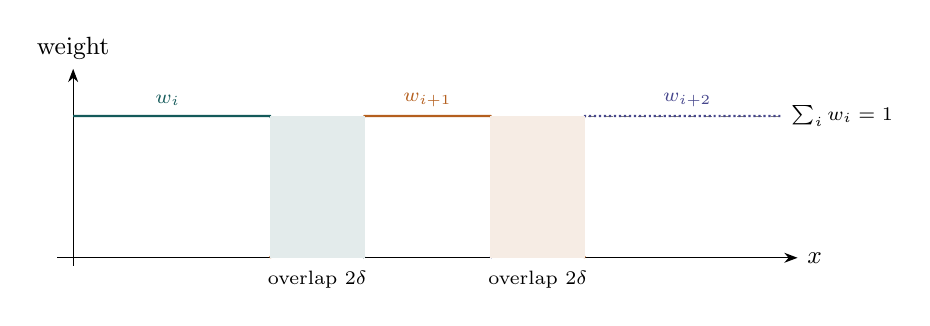
\begin{tikzpicture}[scale=1.0]
  \def\H{1.8}
  \draw[->,>=Stealth] (-0.2,0) -- (9.2,0) node[right,font=\small] {$x$};
  \draw[->,>=Stealth] (0,-0.1) -- (0,2.4) node[above,font=\small] {weight};
  \draw[dashed,gray] (0,\H) -- (9,\H) node[right,font=\scriptsize,black] {$\sum_i w_i = 1$};
  \draw[accent,thick] (0,\H) -- (2.5,\H) -- (3.7,0);
  \draw[accent2,thick] (2.5,0) -- (3.7,\H) -- (5.3,\H) -- (6.5,0);
  \draw[accent3,thick,densely dotted] (5.3,0) -- (6.5,\H) -- (9,\H);
  \fill[accent!12] (2.5,0) rectangle (3.7,\H);
  \fill[accent2!12] (5.3,0) rectangle (6.5,\H);
  \node[font=\scriptsize,accent] at (1.2,\H+0.2) {$w_i$};
  \node[font=\scriptsize,accent2] at (4.5,\H+0.2) {$w_{i+1}$};
  \node[font=\scriptsize,accent3] at (7.8,\H+0.2) {$w_{i+2}$};
  \node[font=\scriptsize,anchor=north] at (3.1,-0.05) {overlap $2\delta$};
  \node[font=\scriptsize,anchor=north] at (5.9,-0.05) {overlap $2\delta$};
\end{tikzpicture}
\caption{\textbf{Partition-of-unity windows along one axis.} Each interior is
extended by the taper width $\delta$ so adjacent Hann windows overlap by $2\delta$;
inside the overlap two windows ramp so their sum stays $1$. Dividing by the overlap
sum makes $\sum_i w_i\equiv 1$ exact, so the merge is a smooth convex blend across
every seam \cite{ronneberger2015unet,bartal2023multidiffusion}.}
\label{fig:pou}
\end{figure}

\subsection{Periodicity}\label{sec:periodic}

The lab's urban LES domains are periodic in the spanwise ($y$) direction, so
periodicity must wrap genuinely rather than clip. An axis is flagged periodic in the
configuration (default $y$). On a periodic axis (Figure~\ref{fig:periodic}):
\begin{itemize}
\item \textbf{Halo wrap.} A boundary tile reads its halo circularly from the
opposite side of the domain, so $\Rop_i$ never invents a wall.
\item \textbf{Partition-of-unity wrap.} The $n+2\delta$ window overhang of a
seam-adjacent tile is \emph{wrap-added} onto the opposite end before the overlap-sum
normalization, so $\sum_i w_i\equiv1$ holds \emph{across} the seam and the merge is
seamless there.
\item \textbf{Positional wrap.} The positional encoding $\bm e_i$
(Section~\ref{sec:fine}) uses a smooth $\sin(2\pi\,\cdot/N)$ signal on a periodic
axis instead of a signed coordinate that would imply a (non-existent) wall.
\end{itemize}
The single constraint is that the interior size $n$ must divide a periodic axis's
length, since such an axis cannot be zero-padded to a multiple of $n$ without
changing its circumference. The inner networks are \emph{not} themselves told about
periodicity: the wrap is already baked into the halo they receive, so they use
ordinary patch-edge padding.

\begin{figure}[t]
\centering
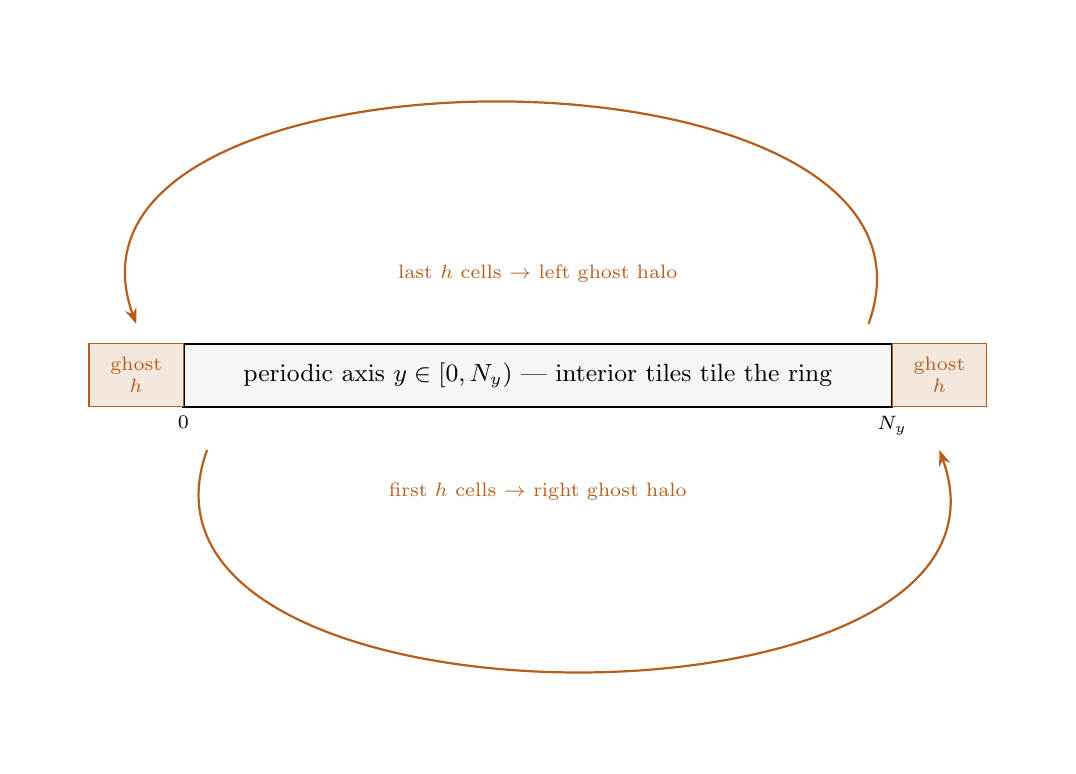
\begin{tikzpicture}[ar/.style={-{Stealth[length=2mm]},thick}]
  \def\L{9}\def\g{1.2}
  \draw[thick,fill=boxbg] (0,0) rectangle (\L,0.8);
  \node[font=\small] at (\L/2,0.4) {periodic axis $y\in[0,N_y)$ --- interior tiles tile the ring};
  \node[anchor=north,font=\scriptsize] at (0,0) {$0$};
  \node[anchor=north,font=\scriptsize] at (\L,0) {$N_y$};
  \draw[fill=accent2!15,draw=accent2] (-\g,0) rectangle (0,0.8);
  \node[font=\scriptsize,accent2,align=center] at (-\g/2,0.4) {ghost\\$h$};
  \draw[fill=accent2!15,draw=accent2] (\L,0) rectangle (\L+\g,0.8);
  \node[font=\scriptsize,accent2,align=center] at (\L+\g/2,0.4) {ghost\\$h$};
  \draw[ar,accent2] (\L-0.3,1.05) to[out=70,in=110,looseness=1.1] (-\g/2,1.05);
  \node[accent2,font=\scriptsize,anchor=south] at (\L/2,1.45) {last $h$ cells $\to$ left ghost halo};
  \draw[ar,accent2] (0.3,-0.55) to[out=-110,in=-70,looseness=1.1] (\L+\g/2,-0.55);
  \node[accent2,font=\scriptsize,anchor=north] at (\L/2,-0.85) {first $h$ cells $\to$ right ghost halo};
\end{tikzpicture}
\caption{\textbf{Periodic wrap-around (shown for $y$).} A seam-adjacent patch reads
its halo circularly --- the last $h$ cells fill the left ghost halo and the first
$h$ cells fill the right one --- so $\Rop_i$ reads true neighbours, not a wall. The
partition-of-unity window overhang is wrap-added across the seam in the same way, so
$\sum_i w_i\equiv1$ holds across $y=N_y\equiv0$ and the merge is seamless there.
Requires $n\mid N_y$.}
\label{fig:periodic}
\end{figure}

% =====================================================================
\section{The coarse global level}\label{sec:coarse}

A purely local patch cannot see beyond its halo, so it cannot represent the
instantaneous global coupling of incompressible flow within one step. The coarse
level supplies that missing global view cheaply. Let $\Rop_H$ average-pool the fine
state by an integer factor $r$ onto a coarse grid of shape
$\lceil N_z/r\rceil\times\lceil N_y/r\rceil\times\lceil N_x/r\rceil$ (each axis is
first padded up to a multiple of $r$, so the division is exact after padding), and
let $\mathcal P_H$ be the matching
(trilinear) prolongation back to the fine grid. A small coarse network $\Gcoarse$
takes one low-resolution step, and its prolongation is the \emph{context} field:
\begin{equation}
\bar{\bm S}_t=\Rop_H\bm S_t,\qquad
\bar{\bm S}_{t+1}=\Gcoarse\!\big(\bar{\bm S}_t,\bm p_t,\Rop_H\bm m\big),\qquad
\bm C_t=\mathcal P_H\,\bar{\bm S}_{t+1}.
\label{eq:coarse}
\end{equation}
Because the coarse grid has $r^3$ fewer cells, this pass is cheap.
Figure~\ref{fig:coarse} traces the resolution changes. The geometry is coarsened by
the \emph{any-fluid} rule, $\Rop_H\bm m=\mathbb{1}[\,\mathrm{avgpool}_r(\bm m)>0\,]$,
so a coarse cell is fluid whenever any fine cell in its block is: this keeps thin
fluid corridors visible to the coarse pressure field, which is the whole point of
the level.

\paragraph{Why a dedicated coarse net.}
In principle the coarse network could reuse the fine weights ($\Psi=\Phi$). In the
implementation the fine net's stem is widened to ingest the context and positional
channels (Section~\ref{sec:fine}) while the coarse net receives none, so their first
layers differ in input shape and cannot share weights directly. We therefore use a
small \emph{dedicated} coarse network by default; weight reuse remains available
only by feeding the coarse net zero-filled context channels and is left as a
non-default option.

\begin{figure}[t]
\centering
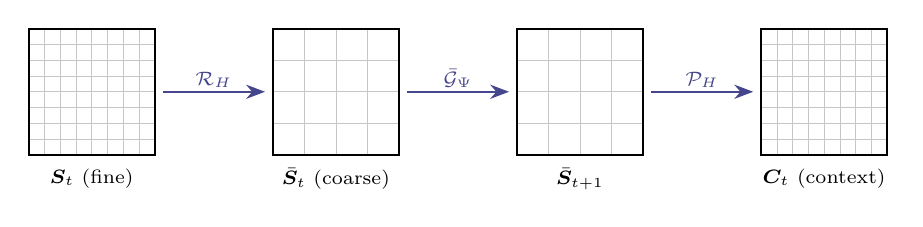
\begin{tikzpicture}[ar/.style={-{Stealth[length=2.4mm]},thick},
  lab/.style={midway,above,font=\scriptsize,fill=white,inner sep=1pt}]
  \def\fine{\draw[step=0.2,gray!45,very thin](0,0)grid(1.6,1.6);\draw[thick](0,0)rectangle(1.6,1.6);}
  \def\coarse{\draw[step=0.4,gray!45,very thin](0,0)grid(1.6,1.6);\draw[thick](0,0)rectangle(1.6,1.6);}
  \begin{scope} \fine \node[font=\scriptsize,anchor=north]at(0.8,-0.05){$\bm S_t$ (fine)}; \end{scope}
  \begin{scope}[xshift=3.1cm] \coarse \node[font=\scriptsize,anchor=north]at(0.8,-0.05){$\bar{\bm S}_t$ (coarse)}; \end{scope}
  \begin{scope}[xshift=6.2cm] \coarse \node[font=\scriptsize,anchor=north]at(0.8,-0.05){$\bar{\bm S}_{t+1}$}; \end{scope}
  \begin{scope}[xshift=9.3cm] \fine \node[font=\scriptsize,anchor=north]at(0.8,-0.05){$\bm C_t$ (context)}; \end{scope}
  \draw[ar,accent3] (1.7,0.8) -- node[lab]{$\Rop_H$} (3.0,0.8);
  \draw[ar,accent3] (4.8,0.8) -- node[lab]{$\Gcoarse$} (6.1,0.8);
  \draw[ar,accent3] (7.9,0.8) -- node[lab]{$\mathcal P_H$} (9.2,0.8);
\end{tikzpicture}
\caption{\textbf{The coarse level.} The fine state is average-pooled by a factor
$r$ to a small coarse grid, a dedicated coarse network takes one step there, and the
result is trilinearly prolonged back to the fine grid as the global context field
$\bm C_t$. The coarse pass costs $r^{3}$ fewer cells than a fine step.}
\label{fig:coarse}
\end{figure}

% =====================================================================
\section{The fine-scale local update}\label{sec:fine}

Each patch receives, channel-wise concatenated: its restricted state $\Rop_i\bm
S_t$ ($C$ channels), its restricted geometry $\Rop_i\bm m$ ($1$ channel), the
restricted coarse context $\Rop_i\bm C_t$ ($C$ channels), and a positional encoding
$\bm e_i$ ($n_{\text{pos}}$ channels: a signed, normalized axis \emph{coordinate}
on non-periodic axes --- monotonic from $-1$ at the low face to $+1$ at the high
face, not a distance to the nearest wall --- and a periodic $\sin$ signal otherwise). The shared fine network
predicts a \emph{residual} (delta-state), which is the standard stable choice for
learned time-steppers:
\begin{align}
\hat{\bm x}_i&=\big[\,\Rop_i\bm S_t\,\Vert\,\Rop_i\bm m\,\Vert\,\Rop_i\bm C_t\,\Vert\,\bm e_i\,\big],
&\Delta_i&=\Gfine(\hat{\bm x}_i,\bm p_t),
&\hat{\bm S}_i&=\big(\Rop_i\bm S_t+\Delta_i\big)\big|_{\Omega_i^\circ}.
\label{eq:fine}
\end{align}
The prediction is computed on the extended block and then cropped to the interior:
halo cells inform the prediction but their own outputs are discarded.

\paragraph{A minimal, back-compatible widening.}
The fine network is the existing \code{UNetConvNeXt}, reused unchanged except for
its input stem. The context and positional channels are extra inputs the original
stem did not expect, so we add an \code{extra\_in\_channels} argument that widens the
stem convolution and concatenates these raw channels right after the geometry
(Figure~\ref{fig:stem}). The extra channels are \emph{not} normalized or
geometry-masked --- the context is already in physical units and the positions are
geometry-independent. With \code{extra\_in\_channels}$=0$ (the default for every
other use of the network) the stem, its parameters, and the saved state-dict keys
are byte-identical to before, so existing checkpoints load unchanged. The residual
head is the network's existing \code{residual=True} mode, and its normalization is
the existing patch-independent (GroupNorm) variant, which avoids the seam artifacts
that batch-dependent normalization would introduce \cite{buglakova2025tiling}.

\begin{figure}[t]
\centering
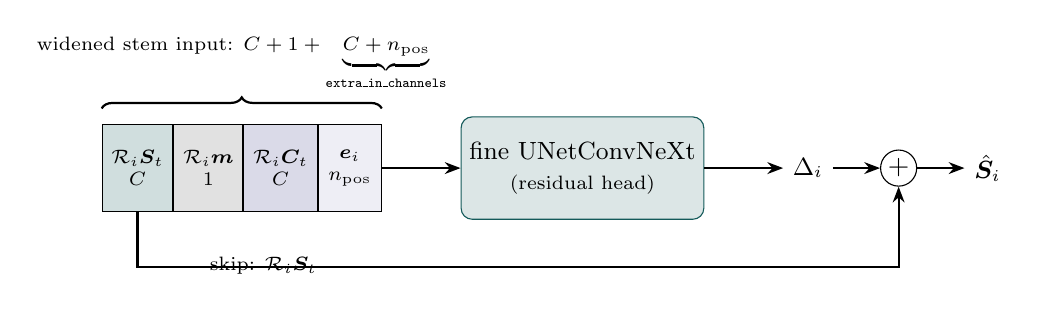
\begin{tikzpicture}[
  ch/.style={draw,minimum width=8mm,minimum height=11mm,font=\scriptsize,align=center},
  ar/.style={-{Stealth[length=2mm]},thick}]
  \node[ch,fill=accent!20] (s) {$\Rop_i\bm S_t$\\$C$};
  \node[ch,fill=solidc!22,right=0pt of s] (g) {$\Rop_i\bm m$\\$1$};
  \node[ch,fill=accent3!20,right=0pt of g] (c) {$\Rop_i\bm C_t$\\$C$};
  \node[ch,fill=accent3!9,right=0pt of c] (e) {$\bm e_i$\\$n_{\text{pos}}$};
  \draw[decorate,decoration={brace,amplitude=4pt},thick]
    ([yshift=2mm]s.north west) -- node[above,yshift=3pt,font=\scriptsize]
    {widened stem input: $C+1+\underbrace{C+n_{\text{pos}}}_{\code{extra\_in\_channels}}$}
    ([yshift=2mm]e.north east);
  \node[net,right=10mm of e,minimum height=13mm] (net) {fine UNetConvNeXt\\\scriptsize (residual head)};
  \draw[ar] (e) -- (net);
  \node[right=10mm of net,font=\small] (d) {$\Delta_i$};
  \draw[ar] (net) -- (d);
  \node[draw,circle,inner sep=1pt,right=6mm of d] (plus) {$+$};
  \draw[ar] (d) -- (plus);
  \draw[ar] (s.south) |- ([yshift=-7mm]s.south) -| (plus);
  \node[font=\scriptsize,anchor=north] at ($(s.south)+(1.6,-0.45)$) {skip: $\Rop_i\bm S_t$};
  \node[right=6mm of plus,font=\small] (sh) {$\hat{\bm S}_i$};
  \draw[ar] (plus) -- (sh);
\end{tikzpicture}
\caption{\textbf{Fine-net input assembly and the widened stem.} Per patch, four
groups of channels are concatenated --- state, geometry, prolonged coarse context,
and positional encoding --- and fed to the shared UNet through a stem widened by
\code{extra\_in\_channels}$=C+n_{\text{pos}}$. The network predicts a residual
$\Delta_i$ added to the patch state to give $\hat{\bm S}_i$. At
\code{extra\_in\_channels}$=0$ the widening is a no-op and the network is identical
to the original.}
\label{fig:stem}
\end{figure}

% =====================================================================
\section{Partition-of-unity merge and the rollout}\label{sec:merge}

The global next state is the windowed sum of the interior predictions,
\begin{equation}
\boxed{\;\bm S_{t+1}=\sum_{i=1}^{M}\Eop_i\!\big(w_i\odot\hat{\bm S}_i\big)\;}
\label{eq:merge}
\end{equation}
where $\odot$ is point-wise multiplication broadcast over channels. By
\eqref{eq:pou}, every cell is a convex combination of the patches covering it;
away from overlaps a single window equals $1$ and the patch is used directly. The
merged field is then multiplied by the geometry mask. Figure~\ref{fig:interface}
shows the overlap band where two interiors blend (and where the training-time
interface penalty of Section~\ref{sec:training} acts).

\begin{figure}[t]
\centering
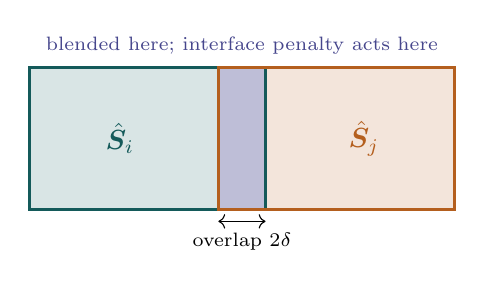
\begin{tikzpicture}
  \fill[accent!16] (0,0) rectangle (3,1.8);
  \fill[accent2!16] (2.4,0) rectangle (5.4,1.8);
  \fill[accent3!35] (2.4,0) rectangle (3,1.8);
  \draw[accent,very thick] (0,0) rectangle (3,1.8);
  \draw[accent2,very thick] (2.4,0) rectangle (5.4,1.8);
  \node[accent] at (1.15,0.9) {$\hat{\bm S}_i$};
  \node[accent2] at (4.25,0.9) {$\hat{\bm S}_j$};
  \draw[<->] (2.4,-0.15) -- (3.0,-0.15);
  \node[font=\scriptsize,anchor=north,align=center] at (2.7,-0.18) {overlap $2\delta$};
  \node[font=\scriptsize,anchor=south,accent3] at (2.7,1.85) {blended here; interface penalty acts here};
\end{tikzpicture}
\caption{\textbf{Where neighbours meet.} Two adjacent interior predictions overlap
by $2\delta$ (indigo band). At inference the partition of unity blends them
smoothly; at training time (path b, Section~\ref{sec:training}) the interface term
penalizes their disagreement on exactly this band.}
\label{fig:interface}
\end{figure}

\paragraph{Optional divergence projection.}
If residual velocity divergence at seams remains a problem after the coarse level,
an inexpensive coarse Helmholtz projection can restore $\nabla\!\cdot\!\bm u=0$ by
solving $\nabla^2\phi=\nabla\!\cdot\!\bm u^\star$ and correcting $\bm u\leftarrow\bm
u^\star-\nabla\phi$. This is wired behind a flag (default off) with a placeholder
identity body; the full solve is left as a drop-in once it is shown to matter on a
held-out rollout.

\paragraph{Inference rollout.}
Algorithm~\ref{alg:rollout} is the full autoregressive rollout. The halo for each
patch is read from the current global field, so neighbour information at step $t$ is
exactly the merged state from step $t-1$ --- no separate boundary buffer is needed.

\begin{algorithm}[t]
\caption{Two-level domain-decomposed rollout (one \code{forward} per step)}
\label{alg:rollout}
\begin{lstlisting}[style=pseudo]
Input: state S0, params {p_t}, geometry m, steps T; fine net G, coarse net Gbar
S <- S0
for t = 0 to T-1 do
    # ---- coarse global context, Eq. (3) ----
    Sbar      <- Restrict R_H (S)               # average-pool by r
    Sbar_next <- Gbar(Sbar, p_t, R_H(m))        # one cheap low-res step
    C         <- Prolong P_H (Sbar_next)        # context on the fine grid
    # ---- fine patches (one batched call), Eq. (4) ----
    X    <- Tile/Pad: concat( R_i(S), R_i(m), R_i(C), e_i )  for all i
    dS   <- Predict G(X, p_t)                   # residual on extended blocks
    Shat <- crop_to_interior( R_i(S) + dS )     # discard halo outputs
    # ---- partition-of-unity merge, Eq. (5) ----
    S    <- Merge  sum_i E_i( w_i * Shat_i )    # then mask by geometry
    emit S as state at time t+1
end for
return trajectory {S_1, ..., S_T}
\end{lstlisting}
\end{algorithm}

% =====================================================================
\section{Training}\label{sec:training}

Two interchangeable routes train the same model. Both are selected through Hydra
configuration groups (Section~\ref{sec:config}); neither requires editing code.

\subsection{Path (a): drop-in mean-squared training}\label{sec:dropin}

Because \code{DomainDecomposed} keeps the standard full-grid contract, it trains
with the \emph{existing, unmodified} trainer on the ordinary one-step dataset under
a plain mean-squared error on the merged prediction. The pushforward curriculum
\cite{brandstetter2022mppde}, learning-rate schedule, mixed precision and
\code{torch.compile} of the existing trainer all apply unchanged. This is the
primary, validated route and the recommended starting point.

\subsection{Path (b): the patch objective}\label{sec:patch}

The richer objective adds three physics/consistency penalties to the one-step term:
\begin{equation}
\mathcal L=
\underbrace{\big\|\hat{\bm S}-\bm S^{\text{ref}}_{t+1}\big\|^2}_{\text{one-step}}
+\lambda_{\mathrm{if}}\!\!\sum_{j\in\mathcal N(i)}\!\!\big\|\hat{\bm S}_i-\hat{\bm S}_j\big\|^2_{\Omega_i\cap\Omega_j}
+\lambda_{\mathrm{div}}\big\|\nabla\!\cdot\!\hat{\bm u}\big\|^2
+\lambda_{\mathrm c}\big\|\bar{\bm S}_{t+1}-\Rop_H\bm S^{\text{ref}}_{t+1}\big\|^2 .
\label{eq:loss}
\end{equation}
Table~\ref{tab:loss} explains the four terms and how
\code{DomainDecomposition\-Loss} computes each. The interface term directly trains
seam consistency; the divergence term is a soft physics regularizer complementing
the coarse level; the coarse term supervises $\Gcoarse$.

\begin{table}[t]
\centering\small
\begin{tabularx}{\textwidth}{@{}l l Y@{}}
\toprule
\textbf{Term} & \textbf{Weight} & \textbf{Computed on} \\
\midrule
one-step & $1$ & MSE of the \emph{merged} next state vs.\ ground truth on fluid cells. \\
interface & $\lambda_{\mathrm{if}}=0.1$ & disagreement of adjacent patches' $(n+2\delta)$ PoU blocks on their $2\delta$ overlap band; $+z/+y/+x$ faces (each shared band once); periodic wrap via the neighbour table. \\
divergence & $\lambda_{\mathrm{div}}=0.01$ & squared $\nabla\!\cdot\!\bm u$ (central differences, $\Delta x=1$) of the merged velocity on fluid cells. \\
coarse & $\lambda_{\mathrm c}=1.0$ & MSE of $\bar{\bm S}_{t+1}$ vs.\ $\Rop_H\bm S^{\text{ref}}_{t+1}$. \\
\bottomrule
\end{tabularx}
\caption{The four terms of the patch objective \eqref{eq:loss} and how
\code{DomainDecompositionLoss} evaluates them. Default weights follow standard
practice: start the interface and divergence penalties small and tune on a held-out
rollout.}
\label{tab:loss}
\end{table}

The interface, divergence and coarse terms couple \emph{neighbouring} patches, which
an isolated per-patch sample cannot supply (its neighbours may fall in a different
minibatch, or be absent). The patch trainer (\code{PatchTrainer}) therefore feeds
\emph{full-field} batches and reads the model's per-patch intermediates through an
optional \code{return\_intermediates} flag on \code{forward} --- so every patch's
neighbours are present at every step. A separate per-patch dataset
(\code{PatchTransitionDataset}) reads the same on-disk layout and is available for
one-step, delta-only patch training where isolated patches suffice; multi-step
\emph{patch} pushforward is out of scope because a patch's halo at $t+1$ depends on
its neighbours' merged interiors, which only the full-field model owns.

% =====================================================================
\section{Software architecture and usage}\label{sec:software}

\subsection{The embedded contract}\label{sec:contract}

The load-bearing design decision is that \code{DomainDecomposed} exposes the same
interface as every other architecture: \code{forward(state, params, geometry)}
returns \code{state\_next}, all on full-grid tensors (Figure~\ref{fig:contract}).
The coarse step, tiling, fine step and merge happen \emph{inside} that call. As a
result the existing trainer, the autoregressive forward model, the ensemble wrapper
and the ensemble-smoother data assimilation all drive the decomposed model
unchanged.

\begin{figure}[t]
\centering
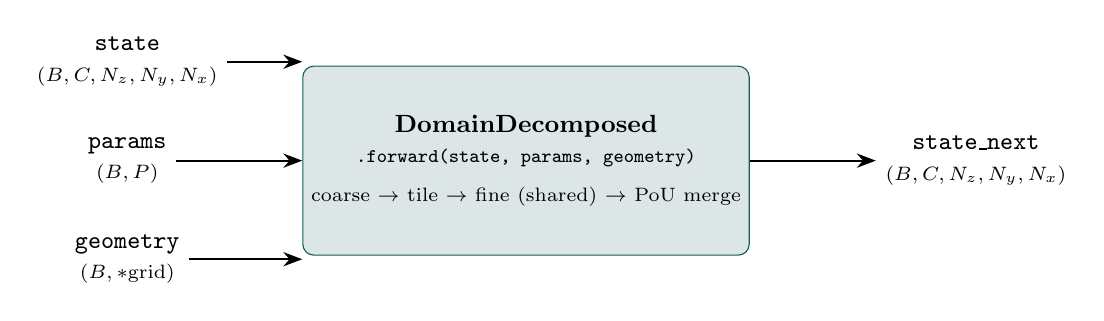
\begin{tikzpicture}[node distance=4mm]
  \node[io] (st) {\code{state}\\\scriptsize$(B,C,N_z,N_y,N_x)$};
  \node[io,below=4mm of st] (pa) {\code{params}\\\scriptsize$(B,P)$};
  \node[io,below=4mm of pa] (ge) {\code{geometry}\\\scriptsize$(B,{*}\mathrm{grid})$};
  \node[net,right=16mm of pa,minimum width=48mm,minimum height=24mm] (M)
     {\textbf{DomainDecomposed}\\\scriptsize\code{.forward(state, params, geometry)}\\[3pt]
      \scriptsize coarse $\to$ tile $\to$ fine (shared) $\to$ PoU merge};
  \node[io,right=16mm of M] (out) {\code{state\_next}\\\scriptsize$(B,C,N_z,N_y,N_x)$};
  \draw[ar] (st.east) -- (st.east -| M.west);
  \draw[ar] (pa.east) -- (M.west);
  \draw[ar] (ge.east) -- (ge.east -| M.west);
  \draw[ar] (M.east) -- (out.west);
\end{tikzpicture}
\caption{\textbf{The decomposition is hidden behind the standard contract.}
\code{forward(state, params, geometry)$\to$state\_next} on full-grid tensors,
byte-for-byte the signature of the other architectures. Trainer, forward model and
ensemble path call it without modification.}
\label{fig:contract}
\end{figure}

\subsection{Flexible global grid}\label{sec:flexible}

Because the trained invariant is the fixed-size patch, not the global grid, one
trained model runs on any grid with the \emph{same cell spacing}
(Figure~\ref{fig:flexible}). The forward model's domain check is relaxed
accordingly: for a domain-flexible model it requires only that the requested cell
spacing $(\Delta x,\Delta y,\Delta z)$ match the trained spacing, instead of
requiring the whole grid to match. The global grid $(N_x,N_y,N_z)$ thus becomes a
free parameter --- the entire point of the decomposition --- while non-decomposed
architectures keep the original strict check.

\begin{figure}[t]
\centering
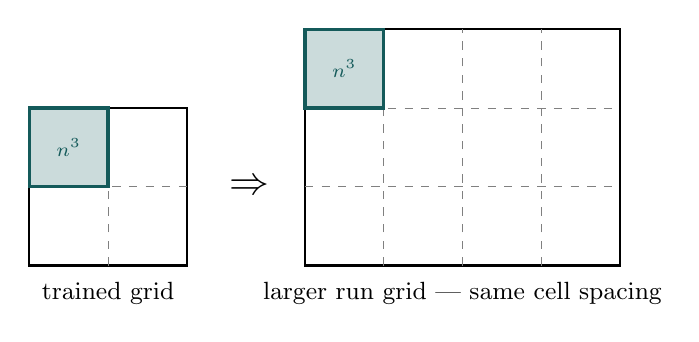
\begin{tikzpicture}[scale=0.5,every node/.style={font=\small}]
  \begin{scope}
    \draw[thick] (0,0) rectangle (4,4);
    \draw[gray,dashed] (2,0)--(2,4); \draw[gray,dashed] (0,2)--(4,2);
    \fill[accent!22] (0,2) rectangle (2,4);
    \draw[accent,very thick] (0,2) rectangle (2,4);
    \node[accent,font=\scriptsize] at (1,3) {$n^3$};
    \node at (2,-0.7) {trained grid};
  \end{scope}
  \node at (5.6,2) {\Large $\Rightarrow$};
  \begin{scope}[xshift=7cm]
    \draw[thick] (0,0) rectangle (8,6);
    \foreach \x in {2,4,6} {\draw[gray,dashed] (\x,0)--(\x,6);}
    \foreach \y in {2,4} {\draw[gray,dashed] (0,\y)--(8,\y);}
    \fill[accent!22] (0,4) rectangle (2,6);
    \draw[accent,very thick] (0,4) rectangle (2,6);
    \node[accent,font=\scriptsize] at (1,5) {$n^3$};
    \node at (4,-0.7) {larger run grid --- same cell spacing};
  \end{scope}
\end{tikzpicture}
\caption{\textbf{Flexible global grid.} The patch size $n$ (with its halo) is the
invariant; the same trained weights tile a larger domain just by adding more
patches. Only the cell spacing must match training; $(N_x,N_y,N_z)$ is free.}
\label{fig:flexible}
\end{figure}

\subsection{Configuration groups and CLI}\label{sec:config}

Architecture, trainer and loss are all Hydra groups, so the two training routes are
selected entirely on the command line (Figure~\ref{fig:training}). The architecture
is chosen at the \code{architectures} group level (value \code{family/preset}) so any
family is swappable; \code{trainer} switches between the generic trainer
(\code{standard}) and the patch trainer (\code{dd\_patch}); \code{loss} switches
between \code{mse} and the four-term \code{dd} loss. The single
\code{architecture.periodic\_axes: [y]} setting drives both a plain UNet and a
decomposed model --- the latter translates it into its decomposition's $(z,y,x)$
periodicity.

\begin{lstlisting}[style=pseudo,xleftmargin=0pt]
# (a) drop-in: generic Trainer + MSE on the full grid (default groups)
train ... 'architectures@architecture=domain_decomposed/small' \
          model_name=dd_small init_weights_path=null

# (b) patch objective: PatchTrainer + DomainDecompositionLoss
train ... 'architectures@architecture=domain_decomposed/small' \
          'trainer@trainer=dd_patch' 'loss@loss=dd' \
          model_name=dd_small init_weights_path=null
\end{lstlisting}

\begin{figure}[t]
\centering
\resizebox{\textwidth}{!}{%
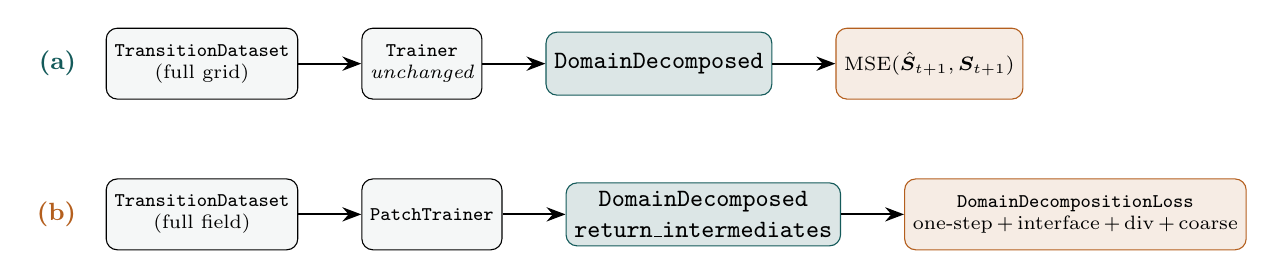
\begin{tikzpicture}[
  bx/.style={draw,rounded corners,align=center,minimum height=9mm,font=\scriptsize,fill=boxbg,inner sep=3pt},
  loss/.style={bx,fill=accent2!12,draw=accent2}]
  \node[bx] (a1) {\code{TransitionDataset}\\(full grid)};
  \node[bx,right=8mm of a1] (a2) {\code{Trainer}\\\itshape unchanged};
  \node[net,right=8mm of a2] (a3) {\code{DomainDecomposed}};
  \node[loss,right=8mm of a3] (a4) {MSE$(\hat{\bm S}_{t+1},\bm S_{t+1})$};
  \draw[ar] (a1)--(a2); \draw[ar] (a2)--(a3); \draw[ar] (a3)--(a4);
  \node[anchor=east,font=\small\bfseries,accent] at ($(a1.west)+(-0.25,0)$) {(a)};
  \node[bx,below=10mm of a1] (b1) {\code{TransitionDataset}\\(full field)};
  \node[bx,right=8mm of b1] (b2) {\code{PatchTrainer}};
  \node[net,right=8mm of b2] (b3) {\code{DomainDecomposed}\\\code{return\_intermediates}};
  \node[loss,right=8mm of b3] (b4) {\code{DomainDecompositionLoss}\\one-step\,$+$\,interface\,$+$\,div\,$+$\,coarse};
  \draw[ar] (b1)--(b2); \draw[ar] (b2)--(b3); \draw[ar] (b3)--(b4);
  \node[anchor=east,font=\small\bfseries,accent2] at ($(b1.west)+(-0.25,0)$) {(b)};
\end{tikzpicture}}
\caption{\textbf{Two training routes, selected as config groups.} (a) the validated
drop-in path through the unmodified trainer with an MSE loss; (b) the patch
objective via \code{PatchTrainer} and \code{DomainDecompositionLoss}, reading the
model's per-patch intermediates on full fields. Path (a) is the default; path (b) is
opt-in.}
\label{fig:training}
\end{figure}

\subsection{Module map}\label{sec:modules}

Figure~\ref{fig:modules} summarizes the files. Teal nodes are new modules; orange
nodes are small, back-compatible edits to existing files.

\begin{figure}[t]
\centering
\resizebox{0.96\textwidth}{!}{%
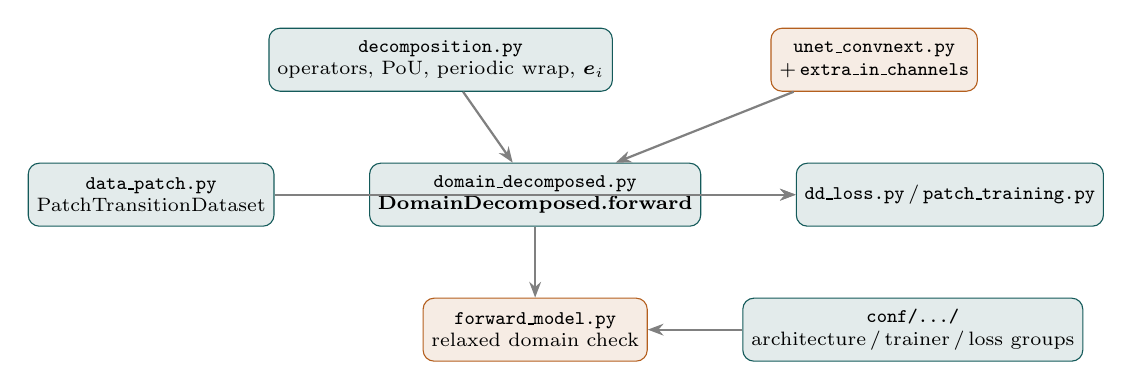
\begin{tikzpicture}[
  file/.style={draw,rounded corners,align=center,font=\scriptsize,fill=boxbg,minimum height=8mm,inner sep=3pt},
  newf/.style={file,fill=accent!12,draw=accent},
  edt/.style={file,fill=accent2!12,draw=accent2},
  gar/.style={-{Stealth[length=2mm]},thick,gray}]
  \node[newf] (dec) {\code{decomposition.py}\\operators, PoU, periodic wrap, $\bm e_i$};
  \node[edt,right=20mm of dec] (unet) {\code{unet\_convnext.py}\\$+$\,\code{extra\_in\_channels}};
  \node[newf,below=9mm of dec,xshift=12mm] (dd) {\code{domain\_decomposed.py}\\\textbf{DomainDecomposed.forward}};
  \node[newf,left=12mm of dd] (data) {\code{data\_patch.py}\\PatchTransitionDataset};
  \node[newf,right=12mm of dd] (loss) {\code{dd\_loss.py}\,/\,\code{patch\_training.py}};
  \node[edt,below=9mm of dd] (fm) {\code{forward\_model.py}\\relaxed domain check};
  \node[newf,right=12mm of fm] (cfg) {\code{conf/\dots/}\\architecture\,/\,trainer\,/\,loss groups};
  \draw[gar] (dec) -- (dd);
  \draw[gar] (unet) -- (dd);
  \draw[gar] (dd) -- (fm);
  \draw[gar] (dd) -- (loss);
  \draw[gar] (data) -- (loss);
  \draw[gar] (cfg) -- (fm);
\end{tikzpicture}}
\caption{\textbf{As-built module map.} Teal = new files; orange = back-compatible
edits. \code{DomainDecomposed} composes the decomposition operators with the
stem-widened UNet; the forward model only relaxes its domain check; the
loss/patch-trainer and the patch dataset form the optional patch-objective path; the
configuration groups wire the choices.}
\label{fig:modules}
\end{figure}

% =====================================================================
\section{Validation}\label{sec:validation}

The implementation ships with unit and integration tests that pin the load-bearing
properties:
\begin{itemize}
\item \textbf{Partition of unity.} $\sum_i w_i\equiv1$ to $10^{-6}$ on several
grids, including non-multiples of $n$ and across a periodic seam; a field smooth
across the $y$-wrap round-trips through tile-then-merge with no seam discontinuity.
\item \textbf{Geometry and operators.} Restriction-then-merge of a constant field is
the identity (within crop); coarsened geometry follows the any-fluid rule; the halo
of a periodic boundary tile equals the wrapped opposite-side cells.
\item \textbf{Back-compatibility.} With \code{extra\_in\_channels}$=0$ the UNet's
state-dict keys and outputs are identical to the original.
\item \textbf{Flexible grid.} A single model instance runs on two different global
grids; obstacle cells are exactly zero in the output; gradients reach both the fine
and coarse networks.
\item \textbf{End-to-end wiring.} The Hydra composition trains, for both routes, a
\code{DomainDecomposed} model through \code{run(cfg)} on a tiny dataset and writes a
loadable checkpoint; the four-term loss drives down on an overfit smoke test.
\end{itemize}

% =====================================================================
\section{Limitations and future work}\label{sec:future}

The coarse network is dedicated rather than weight-shared; sharing would need a
unified stem. The divergence projection is wired but not yet a real solve.
Multi-step \emph{patch} pushforward is unsupported (it needs the full merge each
step); the drop-in path's pushforward curriculum covers multi-step training on the
full field instead. Finally, an exact-tiling variant with consistent halo exchange
\cite{barwey2024consistentgnn,li2020deepddm,huang2025operatorddm} --- which
reproduces a whole-domain rollout seam-free when the halo exceeds the receptive
field, at the cost of giving up the coarse level's global coupling --- is a natural
complement once seam exactness, rather than physics coupling, becomes the binding
constraint. The local receptive field that such a variant requires can be estimated
empirically \cite{ye2024lno}.

\bibliographystyle{plain}
\bibliography{references}

\end{document}
